\documentclass[11pt,letterpaper]{article}
\usepackage[lmargin=1in,rmargin=1in,tmargin=1in,bmargin=1in]{geometry}
\usepackage{../style/homework}
\usepackage{../style/commands}
\setbool{quotetype}{true} % True: Side; False: Under
\setbool{hideans}{false} % Student: True; Instructor: False

% -------------------
% Content
% -------------------
\begin{document}

\homework{10: Due 01/20}{I'm fast. To give you a reference point, I'm somewhere between a snake and a mongoose\dots and a panther.}{Dwight Schrute, The Office}

% Problem 1
\problem{10} Sketch the function $y= 10 \left( \dfrac{1}{2} \right)^x$. 
	\[
	\fbox{
	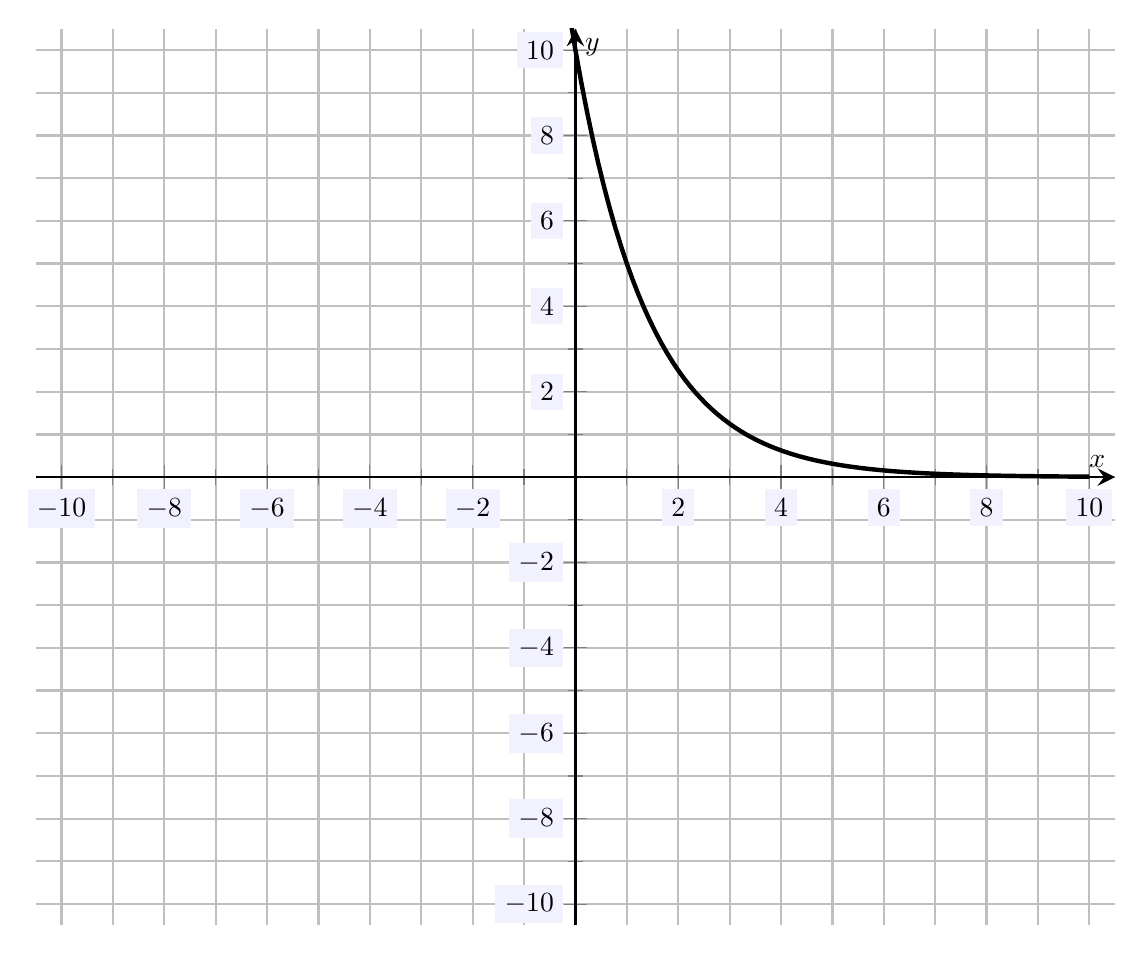
\begin{tikzpicture}[scale=2,every node/.style={scale=0.5}]
	\begin{axis}[
	grid=both,
	axis lines=middle,
	ticklabel style={fill=blue!5!white},
	xmin= -10.5, xmax=10.5,
	ymin= -10.5, ymax=10.5,
	xtick={-10,-8,-6,-4,-2,0,2,4,6,8,10},
	ytick={-10,-8,-6,-4,-2,0,2,4,6,8,10},
	minor tick = {-10,-9,...,10},
	xlabel=\(x\),ylabel=\(y\),
	]
	\addplot[thick, domain= -1:10, samples=100] ({x},{10*(1/2)^x});
	\end{axis}
	\end{tikzpicture}
	}
	\] \pspace

We know that $y(0)= 10 \left( \dfrac{1}{2} \right)^0= 10 \cdot 1= 10$, so that the $y$-intercept is $(0, 10)$. We know also that the function having the form $y= Ab^{cx}$ with $A= 10 > 0$, $b= \frac{1}{2} < 1$, and $c= 1 > 0$, that the function has exponential decay, i.e. is decreasing. This gives the sketch above. Alternatively, we have\dots
	\begin{table}[!ht]
	\centering
	\begin{tabular}{r|rrrrrrrrrrrr}
	$x$ & $-1$ & $0$ & $1$ & $2$ & $3$ & $4$ & $5$ & $6$ & $7$ & $8$ & $9$ & $10$ \\ \hline
	$f(x)$ & $20$ & $10$ & $5$ & $\frac{5}{2}$ & $\frac{5}{4}$ & $\frac{5}{8}$ & $\frac{5}{16}$ & $\frac{5}{32}$ & $\frac{5}{64}$ & $\frac{5}{128}$ & $\frac{5}{256}$ & $\frac{5}{512}$
	\end{tabular}
	\end{table}



\newpage



% Problem 2
\problem{10} Sketch the function $y= 5 - 2^{1 - x}$.
	\[
	\fbox{
	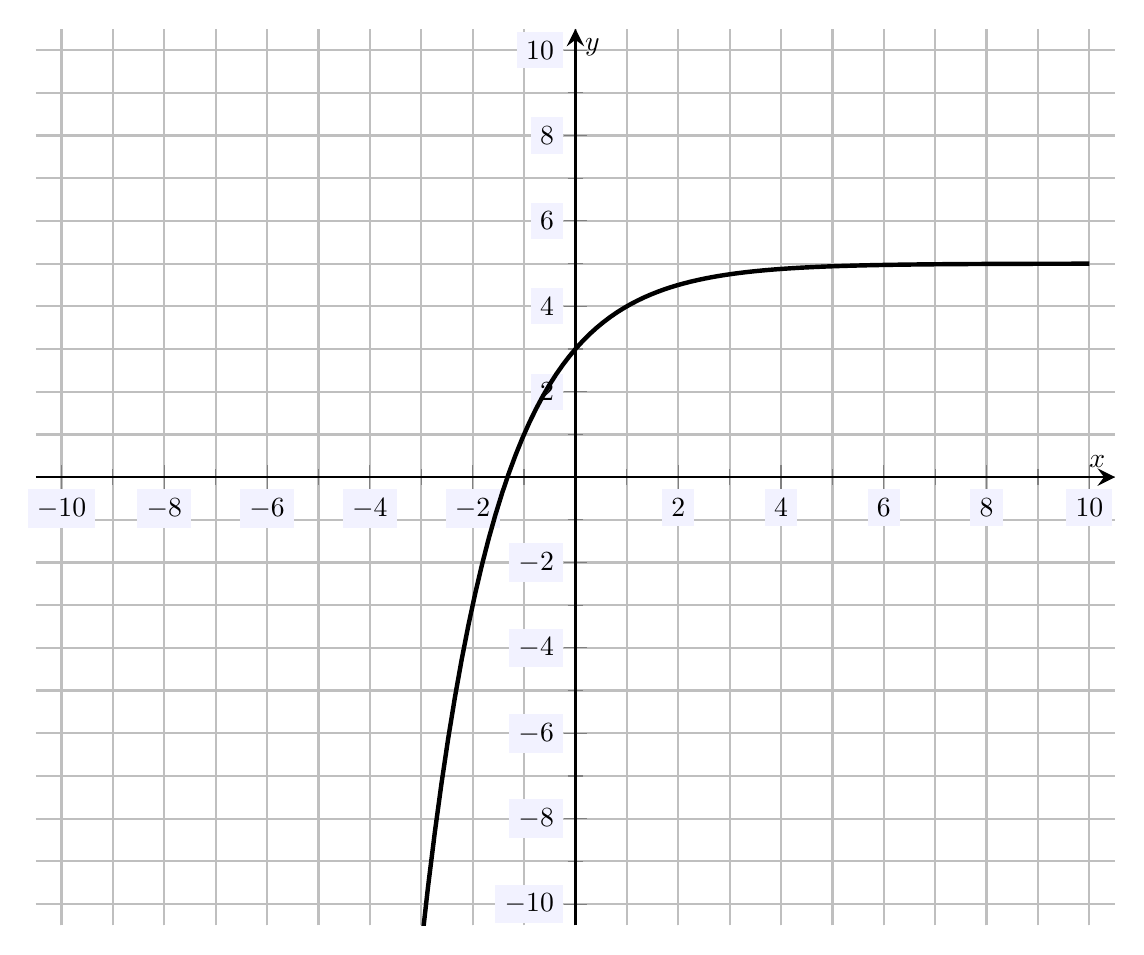
\begin{tikzpicture}[scale=2,every node/.style={scale=0.5}]
	\begin{axis}[
	grid=both,
	axis lines=middle,
	ticklabel style={fill=blue!5!white},
	xmin= -10.5, xmax=10.5,
	ymin= -10.5, ymax=10.5,
	xtick={-10,-8,-6,-4,-2,0,2,4,6,8,10},
	ytick={-10,-8,-6,-4,-2,0,2,4,6,8,10},
	minor tick = {-10,-9,...,10},
	xlabel=\(x\),ylabel=\(y\),
	]
	\addplot[thick, domain= -3:10, samples=100] ({x},{5 - 2^(1 - x)});
	\end{axis}
	\end{tikzpicture}
	}
	\] \pspace

We know that $y(0)= 5 - 2^{1 - 0}= 5 - 2= 3$, so that the $y$-intercept is $(0, 3)$. Rewriting $y$, we find\dots
	\[
	y= 5 - 2^{1 - x}= 5 + (-1) \cdot 2^{1 - x}= 5 + (-1) \cdot 2^1 \cdot 2^{-x}= 5 + (-2) 2^{-x}
	\]
The exponential part of this function has the form $y= Ab^{cx}$ with $A= -2 < 0$, $b= 2 > 1$, and $c= -1 < 0$, that the function is increasing. This gives the sketch above. Alternatively, we have\dots
	\begin{table}[!ht]
	\centering
	\begin{tabular}{r|rrrrrrrrrrrr}
	$x$ & $-4$ & $-3$ & $-2$ & $-1$ & $0$ & $1$ & $2$ & $3$ & $4$ & $5$ & $6$ & $7$ \\ \hline
	$f(x)$ & $-27$ & $-11$ & $-3$ & $1$ & $3$ & $4$ & $\frac{9}{2}$ & $\frac{19}{4}$ & $\frac{39}{8}$ & $\frac{79}{16}$ & $\frac{159}{32}$ & $\frac{319}{64}$
	\end{tabular}
	\end{table}



\newpage



% Problem 3
\problem{10} Write function $f(x)=  2 \left( \dfrac{1}{3} \right)^{2 - x}$ in the form $f(x)= Ab^x$, identifying $A$ and $b$, and determine whether the function $f(x)$ is increasing or decreasing. \pspace

\sol We have\dots
	\[
	\begin{aligned}
	f(x)&= 2 \left( \dfrac{1}{3} \right)^{2 - x} \\[0.3cm]
	&= 2 \cdot \left( \dfrac{1}{3} \right)^2 \cdot \left( \dfrac{1}{3} \right)^{-x} \\[0.3cm]
	&= 2 \cdot \dfrac{1}{9} \cdot \left( \dfrac{1}{3} \right)^{-x} \\[0.3cm]
	&= \dfrac{2}{9} \cdot \left(\left( \dfrac{1}{3} \right)^{-1} \right)^x \\[0.3cm]
	&= \dfrac{2}{9} \cdot 3^x 
	\end{aligned}
	\] \pspace
Then $f(x)= \frac{2}{9} \cdot 3^x$ has the form $f(x)= Ab^x$ with $A= \frac{2}{9}$ and $b= 3$. Because this is a general exponential function $Ab^{cx}$ with $A= \frac{2}{9} > 0$, $b= 3 > 1$, and $c= 1 > 0$, we know that $f(x)$ is increasing. 



\newpage



% Problem 4
\problem{10} Write function $f(x)= -5(2^{3x})$ in the form $f(x)= Ab^x$, identifying $A$ and $b$, and determine whether the function $f(x)$ is increasing or decreasing. \pspace

\sol We have\dots
	\[
	\begin{aligned}
	f(x)&= -5(2^{3x}) \\[0.3cm]
	&= -5 \cdot (2^3)^x \\[0.3cm]
	&= -5(8^x)
	\end{aligned}
	\] \pspace
Then $f(x)= -5(8^x)$ has the form $f(x)= Ab^x$ with $A= -5$ and $b= 8$. Because this is a general exponential function $Ab^{cx}$ with $A= -5 < 0$, $b= 8 > 1$, and $c= 1 > 0$, we know that $f(x)$ is decreasing. 



\newpage



% Problem 5
\problem{10} Write function $f(x)=  6 - 2^{1 - 2x}$ in the form $f(x)= Ab^x + C$, identifying $A$, $b$, and $C$, and determine whether the function $f(x)$ is increasing or decreasing. \pspace

\sol We have\dots
	\[
	f(x)=  6 - 2^{1 - 2x}= 6 - 2 \cdot 2^{-2x}= 6 - 2 \cdot (2^{-2})^x= 6 - 2 \cdot \left( \dfrac{1}{2^2} \right)^x= 6 - 2 \left( \dfrac{1}{4} \right)^x= - 2 \left( \dfrac{1}{4} \right)^x + 6
	\]
Therefore, the function $f(x)$ has the form $f(x)= Ab^x + C$ with $A= -2$, $b= \frac{1}{4}$, and $C= 6$. Because the exponential part of this function has the form $y= Ab^{cx}$ with $A= -2 < 0$, $b= \frac{1}{4} < 1$, and $c= 1 > 0$, we know that $f(x)$ is increasing. 



\newpage



% Problem 6
\problem{10} Consider the function $y= -25 (5^{-3x})$.
        \begin{enumerate}[(a)]
        \item Is the function increasing or decreasing? Explain.
        \item Find the $y$-intercept of this function.
        \item What are the $x$-intercepts and zeros for this function?
        \item Find $y(-1)$. 
        \end{enumerate} \pspace

\sol
\begin{enumerate}[(a)]
\item We have\dots
	\[
	y= -25 (5^{-3x})= -25 \cdot (5^{-3})^x= -25 \left( \dfrac{1}{5^3} \right)^x= -25 \left( \dfrac{1}{125} \right)^x 
	\]
Because this function has the form $f(x)= Ab^{cx}$ with $A= -25 < 0$, $b= \frac{1}{125} < 1$, and $c= 1 > 0$, we know that $y$ is an increasing function. \pspace

\item The $y$-intercept occurs when $x= 0$, but then\dots
	\[
	y(0)= -25(5^{-3 \cdot 0})= -25 (5^0)= -25 \cdot 1= -25
	\]
Therefore, the $y$-intercept is $(0, -25)$. \pspace

\item The $x$-intercepts occur at zeros for $y(x)$. The zeros are the $x$-values such that $y(x)= 0$. But then we have\dots
	\[
	\begin{aligned}
	-25(5^{-3x})&= 0 \\
	5^{-3x}&= 0
	\end{aligned}
	\]
But because $5^{-3x} > 0$ for all $x$, we know that $5^{-3x} \neq 0$. Therefore, $y(x)$ has no zeros. But then $y(x)$ also has no $x$-intercepts. \pspace

\item We have\dots
	\[
	y(-1)= -25(5^{-3 \cdot -1})= -25 (5^3)= -25 (125)= -3125
	\]
\end{enumerate}



\newpage



% Problem 7
\problem{10} Showing all your work, solve the following equation:
	\[
	3^{1 - x}= 27
	\] \pspace

\sol We have\dots
	\[
	\begin{aligned}
	3^{1 - x}&= 27 \\[0.3cm]
	3^{1 - x}&= 3^3
	\end{aligned}
	\]
Comparing powers, this implies that $1 - x= 3$. But then $x= 1 - 3= - 2$. 



\newpage



% Problem 8
\problem{10} Showing all your work, solve the following equation:
	\[
	64^x= \dfrac{1}{2}
	\] \pspace

\sol We have\dots
	\[
	\begin{aligned}
	64^x&= \dfrac{1}{2} \\[0.3cm]
	64^x&= 2^{-1} \\[0.3cm]
	(2^6)^x&= 2^{-1} \\[0.3cm]
	2^{6x}&= 2^{-1}
	\end{aligned}
	\]
Comparing powers, we have $6x= -1$, which implies $x= -\frac{1}{6}$. 



\newpage



% Problem 9
\problem{10} Showing all your work, solve the following equation:
	\[
	2\left( \dfrac{1}{3} \right)^{-x} - 59= -5
	\] \pspace

\sol We have\dots
	\[
	\begin{aligned}
	2\left( \dfrac{1}{3} \right)^{-x} - 59&= -5 \\[0.3cm]
	2\left( \dfrac{1}{3} \right)^{-x}&= 54 \\[0.3cm]
	\left( \dfrac{1}{3} \right)^{-x}&= 27 \\[0.3cm]
	(3^{-1})^{-x}&= 27 \\[0.3cm]
	3^x&= 3^3
	\end{aligned}
	\]
Comparing powers, we see that $x= 3$. 



\newpage



% Problem 10
\problem{10} Showing all your work, solve the following equation:
	\[
	2^{3x} - 7= 9
	\] \pspace

\sol We have\dots
	\[
	\begin{aligned}
	2^{3x} - 7&= 9 \\[0.3cm]
	2^{3x}&= 16 \\[0.3cm]
	2^{3x}&= 2^4
	\end{aligned}
	\]
Comparing powers, we find that $3x= 4$, which implies that $x= \frac{4}{3}$. 


\end{document}